\documentclass[output=paper]{langsci/langscibook} 
\ChapterDOI{10.5281/zenodo.2579045}
\author{Miryam de Lhoneux\affiliation{Uppsala University}\and Omri Abend \affiliation{Hebrew University of Jerusalem}\lastand Mark Steedman \affiliation{University of Edinburgh}}
\title{Investigating the effect of automatic MWE recognition on CCG parsing}
\abstract{We investigate the use of automatic Multiword Expressions (MWEs) recognition in parsing with Combinatory Categorial Grammar. We transform the representation of MWEs in CCGbank by collapsing them to one token. Our model significantly outperforms the baseline on the transformed gold standard showing the benefit of having this information at training time. It also performs significantly better on the transformed gold standard when the transformation is done before parsing as opposed to after parsing which shows that it can help the parser at prediction time. We conclude that despite the limited settings (our transformation algorithm is only able to deal with MWEs that do not cross constituent boundaries), our method can lead to improvements. We obtain different results with MWE recognisers that detect different types of MWE and therefore emphasize the need to experiment with different recognisers to find out which ones this method is best suited to.}

\maketitle

\begin{document}

\section{Introduction}
\label{del:introduction}

\subsection{Motivation}
\indent \isi{Multiword Expressions} (henceforth MWE(s)) are increasingly receiving attention in NLP. They represent a wide variety of phenomena with different properties but are generally agreed to be a group of multiple lexemes which have some level of \isi{idiomaticity} or irregularity \citep{sag02}. They represent varied phenomena but, due to this irregularity, they are all generally considered a problem for NLP tasks and they are often a problem for \isi{syntactic parsing}. \\
\indent Recent research is showing that information about MWEs can help the \isi{syntactic parsing} task \citep{nivre2004multiword,korkontzelosetal2010} and inversely, information about syntactic analysis helps MWE identification \citep{green13,weller&heid2010,martens&vandeghinste2010}. Working on either of the tasks by using information from the other has thus proven to be a useful thing to do and adding MWE information to the \isi{syntactic parsing} task has proven useful in that it has helped increase parsing accuracy. Work on adding MWE information to \isi{syntactic parsing} so far has been restricted to certain types of MWEs (multiword nouns, numerical expressions and compound function words in \citet{nivre2004multiword}, compound nominals, proper names and adjective-noun constructions in \citet{korkontzelosetal2010}) and hence leaves room for improvement.\\
\indent Combinatory Categorial Grammar (henceforth \isi{CCG}) is a strongly lexicalized formalism that is increasingly being used for parsing in NLP applications because of its computational and linguistic properties and because \isi{CCG} parsers perform relatively well on the Penn Treebank (PTB). To give just a few examples, \isi{CCG} is used in Machine Translation \citep[e.g.][]{birch2007ccg}, sentence realization \citep[e.g][]{white2006efficient}, semantic parsing and language acquisition \citep[e.g.][]{krishnamurthy2012weakly}, open-domain question answering and entailment \citep[e.g.][]{lewis2013combining}.\\
\indent For these reasons, \isi{CCG} parsing is an ideal framework to carry on the work on the interaction between \isi{syntactic parsing} and \isi{MWEs} and because \isi{CCG} is a lexicalized formalism and thus encodes a lot of information in the lexicon, it would be useful to work on it by providing it with information about MWEs. 

\subsection{Aims}
\indent No work so far has tried to use MWE information to improve \isi{CCG} parsing which is what we intend to do in this work. Different approaches to using MWE information for improving \isi{syntactic parsing} have been conducted so far with different syntactic models. We conduct one of them which will be argued to be far from ideal but a necessary first step useful to build a sound baseline. The approach we pursue consists in altering training and test data, i.e. transforming the representation of MWEs so that they form one lexical item in them (and hence retokenize the sentence). We experiment with different \isi{MWE recognition} methods so as to find out if the approach works better with certain types of MWEs than with others.\\
\indent The two research questions we therefore try to answer are first whether or not we can improve \isi{CCG} parsing with MWEs and second whether or not applying the same transformation approach to different types of MWEs can lead to different results.

\subsection{Overview of the chapter}
\indent We give an overview of the background literature to further support our motivations and elaborate on the research questions in Section~\ref{del:relatedwork}. We then explain and motivate the methodology we propose to use in order to answer the research questions in Section~\ref{del:methodology}. We present our experiments and results in Section~\ref{del:exp}. We conclude from our study and propose avenues of research in Section~\ref{del:ccl}.


\section{Background}
\label{del:relatedwork}

\subsection{Multiword expressions}
\label{del:MWEs}
\indent \isi{MWEs} is an umbrella term that has been used to characterize a wide variety of phenomena. The most commonly acknowledged definition of this term since \citet{sag02} is that it is a group of multiple lexemes which have some level of \isi{idiomaticity} or irregularity. The multiple lexemes in a MWE are called MWE units in the remainder of this chapter for convenience. This \isi{idiomaticity} may be lexico-syntactic such as in the unusual coordination of a preposition and an adjective in \textit{by and large}. It may be semantic such as in the idiom \textit{kick the bucket} in which the meaning of the whole is not dividable into the meaning of the parts. It may be pragmatic such as in \textit{good morning} which has a meaning attached to the situation in which it is said. Finally, it may be statistical such as the collocation \textit{strong coffee} in which both units occur more frequently than expected.\\
\indent Different MWE types present different properties. They vary in \isi{flexibility}:\linebreak words may appear between the units of a flexible collocation (\textit{strong home-made coffee}, for example) but not between the units of a lexically fixed figurative expression such as \textit{it's raining cats and dogs}. They also vary in compositionality: \textit{Strong coffee} is fully compositional whereas \textit{kick the bucket} is not and \textit{spill the beans} is semantically decomposable, i.e. the meaning of the whole is not predictable from the meaning of the parts but can be decomposed into its parts: if \textit{spill} is interpreted as \textit{reveal} and \textit{the beans} as \textit{the secret} \citep{nunberg94}.
Despite these varied properties they are all generally agreed to be hard to deal with in NLP applications \citep{sag02} and the importance of dealing with them properly has been increasing over the past decade. As described at length in \citepos{kim2008} thesis, ``dealing with'' MWEs consists in developing systems and models for various kinds of tasks. For syntactic analysis, it is important to identify them in text and extract them to a dictionary. For semantic understanding, it is important to measure their compositionality, classify and interpret them.


\subsection{Combinatory Categorial Grammar}\label{del:CCG}
\subsubsection{Presentation}
Combinatory Categorial Grammar \citep{steedman2000} is a strongly lexicalized\linebreak grammar formalism which is currently gaining popularity in the NLP community.\\
\indent \isi{CCG} was built with the intent of being linguistically aware as well as computationally tractable partly as a reaction to transformationalist ideas which were predominant in formal grammars at the time. It differs from the latter mainly in having one component including syntactic and semantic information instead of having separate modules for each in the \isi{grammar}. Similarly, instead of having a large amount of rules and a lexicon as is the case in traditional grammars, it has a small set of universal rules and a lexicon which encodes most syntactic information.
For the sentence \textit{John buys shares}, a traditional \isi{grammar} has information in the lexicon: that \textit{John} is an NP, that \textit{buys} is a verb, that \textit{shares} is an NP, and in the \isi{grammar}: that a V and an NP form a VP and that an NP and a VP form a sentence S, as in Figure~\ref{del:fig:1}.
By contrast, for the same sentence, \isi{CCG} has information in its lexicon that \textit{John} is an NP, that \textit{shares} is an NP and that \textit{buys} first takes an NP to its right then an NP to its left to form a sentence S, as in Figure~\ref{del:fig:2}.\\

\begin{minipage}{.9\textwidth}
\begin{multicols}{2}
    \begin{figure}[H]
        {\small
        \Tree [.S [.NP John ] [.VP [.V buys ] [.NP shares ] ] ]}
        \caption{PTB-style tree\label{del:fig:1}}
    \end{figure}
    \columnbreak
    \begin{figure}[H]
        {\small
        \Tree [.S [.NP John ] [.S\textbackslash NP [.(S\textbackslash NP)/NP buys ] [.NP shares ] ] ]}
        \caption{CCG tree\label{del:fig:2}}
    \end{figure}
\end{multicols}
\vspace{0.6cm}
\end{minipage}

\indent Without going into too much detail about how this works, lexical categories work either as functor or as argument and a set of combinatory rules allow them to combine. For example, the category (S\textbackslash NP)/NP works as a functor that takes an NP to the right (indicated by the forward slash followed by an NP). The category of \textit{buys} therefore can combine with the category of \textit{shares} to result in the category S\textbackslash NP which in turns takes an NP argument to the left (indicated by the backslash followed by an NP), which it finds in the category of \textit{John} to form a sentence S.\\
\indent This \isi{grammar} architecture allows \isi{CCG} to deal elegantly with long-range dependencies. Instead of adding a level of representation in the form of a trace as in Figure~\ref{del:fig:3}, the \isi{grammar} has universal rules which allow the combination of lexical items, as shown in Figure~\ref{del:fig:4}. This has computational advantages and linguistic plausibility: linguistics is increasingly adopting a view of \isi{grammar} where syntax and the lexicon are two modules that are not completely separate in the \isi{grammar} but instead interact with each other. It is a tenet of the recently emerging framework of Construction Grammar \citep{hoffmann2013}. These linguistic and computational properties have made it a widely used framework across NLP research.
\begin{figure}[h]
    \begin{tikzpicture}[scale=.9]
    \Tree [.NP [.NP [.Det A ] [.NP man ] ] [.CP
        [.NP_i whom ] [.TP
            [.NP  I  ] [.VP think  [.TP
                [.NP that [.NP Dexter ] ] [.VP likes [.NP t_i ] ] ] ] ] ] ] 
            \end{tikzpicture}
\caption{PTB-style tree\label{del:fig:3}}
\end{figure}

\begin{figure}[h]
    \begin{tikzpicture}[scale=.9]
    \Tree [.NP [.NP [.NP/N A ] [.N man ] ]  [.NP\textbackslash NP
        [.(NP\textbackslash NP)/(S/NP) whom ] [.S/NP
            [.S/(S\textbackslash NP)  [.NP I ]  ] [.(S\textbackslash NP)/NP [.(S\textbackslash NP)/S think ]  [.S/NP
                [.S/(S\textbackslash NP) [.NP [.NP/N that ] [.N Dexter ] ] ] [.(S\textbackslash NP)/NP likes ] ] ] ] ] ]
            \end{tikzpicture}
\caption{CCG tree\label{del:fig:4}} 
\end{figure}

                        \subsubsection{\isi{CCG} parsing}
                        \indent The first efficient statistical model was the generative model built by \citet{hockenmaier2002} and extended to a discriminative model by \citet{clarkcurran2007}. Both use CCGbank \citep{hockenmaier2007}, a \isi{CCG} converted version of the PTB. Both models perform close to state-of-the-art although with simpler statistical models which is argued by the authors to be the result of having a more expressive \isi{grammar} than the PCFGs used by state-of-the-art parsers.

                        \subsection{Syntactic parsing and multiword expressions}
                        \label{del:syntacticparsingandMWES}
                        \indent As mentioned in Section~\ref{del:MWEs}, the identification of MWEs is important for syntactic analysis. Because they have unusual properties, however, their analysis can be quite problematic. The question of how to deal with MWEs for \isi{syntactic parsing} has been raised by many researchers. It has been approached in different ways. Researchers working with precision grammars such as HPSG for example have accommodated the lexical entries for MWEs in the lexicon so that MWEs are not a problem for parsing. Researchers on data-induced grammars have accommodated the testing and/or training data before parsing. Recent research has proposed to both change the lexicon and the parsing algorithm. A last recent approach is to learn MWE representations and dependency trees jointly. We briefly describe each of these approaches in turn. We describe the second approach in more details than the other two because this is the one we use in this work for reasons explained in Section~\ref{del:app}.

                        \subsubsection{Transforming the lexicon}
                        \indent Different types of lexical entries have been proposed for MWEs in the \isi{grammar}. A lot of research proposes to simply analyse all MWEs as ``words-with-spaces'', i.e.\ group the MWE units together in the syntactic analysis. This analysis has been argued against by many. \citet{sag02} have suggested sophisticated ways of representing the different MWE types in a \isi{grammar}, which have been partly implemented within the framework of the precision \isi{grammar} HPSG, as described by \citet{copestakeetal2002}. \citet{zhangetal2006} established that MWEs are a tremendous source of parse failures when parsing with a precision \isi{grammar} such as HPSG and henceforth proposed a way of using this information to identify new MWEs and enrich a lexicon: they suggested using parse failures to predict the existence of a MWE.

                        \subsubsection{Transforming the data}
                        \label{del:changingdata}
                        \indent Since the seminal work of \citet{nivre2004multiword}, research has shown that treating MWEs as one token or a ``word-with-spaces'' in test and/or in training data before parsing and/or training leads to an improvement in parsing accuracy. \citet{nivre2004multiword} have shown that to be true for deterministic \isi{dependency parsing} and \citet{korkontzelosetal2010} have shown that to be true for shallow parsing. \\
                        \indent The approaches adopted in these two papers are quite different and we describe each in turn.
                        \subsubsubsection{Transforming training and test data}
                        \indent \citet{nivre2004multiword} created two versions of a treebank, one in which MWEs are annotated as if compositional and one in which they are joined as one lexical item. They show that training a parser on the second version of the treebank leads to a better parsing accuracy. They use a corpus with manual MWE annotation to create both versions of the treebank and hence simulate ``perfect'' \isi{MWE recognition}. MWE annotation, however, only consists in a few MWE types so it is not comprehensive. They report improvement in parsing accuracy of the MWEs themselves but also of their surrounding \isi{syntactic structure}. They opened the gate for improving \isi{syntactic parsing} with MWE information but left many questions unanswered. For example, the question of whether or not their results port to other \isi{syntactic parsing} models, whether or not the full potential they obtained with ``perfect'' recognition of MWEs can be obtained with an automatic recogniser and whether or not this potential can be increased when recognising other types of MWEs. Some of these questions have been partially addressed since then. \citet{constant12acl} have shown that with an automatic recogniser, the parsing accuracy improvement is not as dramatic as predicted by \citet{nivre2004multiword}. \citet{eryigit:2011:multiword} found out that in the case of a morphologically rich language (e.g., Turkish), the approach works with some types of MWEs but not with others.
                        \subsubsubsection{Transforming test data}
                        \label{del:korkontz}
                        \indent \citet{korkontzelosetal2010} reported similar parsing accuracy improvements for shallow parsing, showing that \citet{nivre2004multiword}'s results do seem to port to at least one other parsing model. Their technique is, however, quite different. They created a corpus containing a large number of pre-selected MWEs (randomly chosen from WordNet) and converted it to a version in which the MWE units are collapsed to one lexical item. They POS-tag the two versions of the corpus before parsing each. They subsequently analyse the differences in output. In order to do so, they randomly select a sample of output from both parsed corpora and build a taxonomy of changes they observe from one to the other. For each class in the taxonomy, they determine whether the change in output led to increased accuracy, decreased accuracy or did not change the accuracy. They automatically classify the rest of the output data and observe an overall increase in accuracy. Their work not only confirms the results obtained from previous work but also provides an insightful qualitative analysis of changes obtained with their method. They believe the improvement in accuracy is partly due to the fact that the parsing model backs off to POS-tags for rare and unseen words. When MWE units are collapsed to one token, that token is not known by the parser but it still gets assigned a sensible POS-tag because the POS-tagger uses contextual information. 
                        \subsubsection{Transforming the lexicon and the parsing algorithm}
                        \indent A lot of work has shown that although MWE information improves \isi{syntactic parsing}, the reverse is also true: syntactic analysis improves MWE identification. \citet{green13} successfully tuned a parser for MWE identification, \citet{weller&heid2010} and \citet{martens&vandeghinste2010} showed that using parsed corpora for MWE identification is beneficial. These findings led \citet{seretan2013} to propose that neither accommodating the \isi{grammar} with MWE information, nor recognising MWEs in raw text as a help to parsing are appropriate ways of dealing with the issue of MWEs in \isi{syntactic parsing} because neither approach takes advantage of the fact that MWE information and syntactic analysis are mutually informative. She proposes instead to have a MWE lexicon and to deal with potential MWEs during parsing.

                        \subsubsection{Joint learning of MWE identification and parsing}
                        \indent Based on the same observation that the tasks of MWE identification and parsing can inform each other, \citet{constantnivre16} propose to learn both jointly. They use corpora that both have dependency and MWE annotations and modify the parsing algorithm so as to learn both representations jointly. They show that this approach is effective. 

                        \subsubsection{Advantages and caveats of the different approaches}
                        \indent All of these researchers have shown the importance of MWEs for \isi{syntactic parsing} but all of the approaches presented have caveats. Research on HPSG seems to have found the most sophisticated methods of dealing with MWEs but parsing with precision grammars is known to be much less robust \citep{zhang08robustparsing} than parsing with data-induced grammars which make it a suboptimal solution for practical parsing. Learning MWE representations and \isi{syntactic parsing} jointly is probably the most promising approach but it requires a lot of manual work since it requires a corpus that is annotated both with MWEs and dependency trees. As far as other solutions are concerned, they are often very much limited by the type of MWEs that have been dealt with. All other solutions presented as a matter of fact concentrate on a few types of MWEs. However, as argued by \citet{kim2008}, because of the different but interrelated properties of MWEs, it is neither appropriate to try and generalize from MWEs and find a single representation which works for all types, nor is it appropriate to deal with each MWE type at a time. An approach for improving \isi{syntactic parsing} on all MWE types is still lacking and previous approaches leave the question of whether the results can be reproduced with different types of MWEs unanswered. 

                        \subsection{Research questions and objectives}
                        \label{del:relworkccl}
                        \indent  In Section~\ref{del:syntacticparsingandMWES}, it was said that MWE identification information improves \isi{syntactic parsing} although current approaches to doing so leave room for improvement. Trying to improve \isi{syntactic parsing} with MWE information therefore looks like a promising avenue of research. In Section~\ref{del:CCG}, arguments for working with \isi{CCG} parsing were put forward.\\
                        \indent Very little attention has, however, been given to MWEs in \isi{CCG} parsing. \citet{constablecurran} modified CCGbank to have a better representation of verb-particle constructions but did not report any parsing accuracy improvement. No work has tried to establish whether \isi{CCG} parsing accuracy could be improved by adding information about MWEs which is what we intend to do in this work. Our aim is twofold: we want to find out whether or not MWE information can improve \isi{CCG} parsing and we wish to find out if using methods that have been used for a restricted set of types of MWEs can be extended to different types of MWEs. 

\section{Methodology}
\label{del:methodology}

\subsection{Approach}
\label{del:app}
\indent As explained in the last section, in this work we concentrate on an approach that consists in transforming the representation of MWEs in \isi{treebanks}.  In Section~\ref{del:changingdata}, two different versions of this kind of approach have been described. In the first, manual annotation is used to create two versions of the treebank. This left questions unanswered, two of which being whether or not the approach can work with automatic recognition and whether or not the approach can work with different types of MWEs. In this work, we conduct the type of approach described by \citet{nivre2004multiword} using an automatic recogniser to answer the first of these questions in the context of \isi{CCG} parsing. We also experiment with the recogniser by using different versions of it to answer the second of these two questions. This approach is especially interesting in that, as has been shown in \citet{schneider14mwe} who attempted a comprehensive annotation of MWEs in a corpus, even manual annotation of MWEs is a difficult task and experimenting with different MWE recognisers could lead to interesting results.\\ 
\indent Our approach therefore involves transforming both training and test data. Tra\-nsforming the training data can help the parsing model learn more sensible representations of language. For example in the tree for \textit{part of speech}, \textit{of speech} is considered a modifier of \textit{part} as in Figure~\ref{del:fig:pos} which does not make much sense. Instead, grouping the three lexical items as in Figure~\ref{del:fig:pos2} gives a better representation of this group of words. 
\begin{figure}[h]
    \Tree [.NP [.NP Part ] [.NP\textbackslash NP [.(NP\textbackslash NP)/NP of ] [.NP Speech ] ] ]
    \caption{Traditional tree for \textit{Part of Speech}\label{del:fig:pos}}
\end{figure}

\begin{figure}[h]
    \Tree [.NP \qroof{Part of Speech}. ]
    \caption{Tree for \textit{Part of Speech} where tokens are grouped \label{del:fig:pos2}}
\end{figure}

\indent Transforming the test data by for example collapsing the three lexical items \textit{part}, \textit{of} and \textit{speech} to one token \textit{part+of+speech} can help the parser make sensible decisions locally by telling it to consider the three words as one. For example, if this token is followed by a coordinator, the parser knows that coordinating one of the units is not a possibility. In the sentence \textit{it gives part+of+speech and lemma information}, the parser cannot coordinate \textit{speech} with \textit{lemma} which would be a possibility otherwise. Transforming MWEs in training and test data leads to two different effects of adding MWE information to the \isi{syntactic parsing} pipeline and it is best if we can differentiate both in the experiments. We call the first type of effect \textit{training effect} and the second \textit{parsing effect}. We repeat the definition of these two effects below.
    \begin{description}
        \item[Training effect:] the parser learns more sensible representations of MWEs and its units. 
        \item[Parsing effect:] the parser is helped locally in its decision by considering the\linebreak MWE units as one unit.
    \end{description}

\subsection{Parsing model}
\label{del:parsingmodel}
\indent As mentioned in Section~\ref{del:CCG}, both generative and discriminative models exist for parsing with \isi{CCG}. There are different generative models with different properties. We chose to use StatOpenCCG, developed by \citet{christodoulopoulos2008} and recently further expanded by \citet{deoskar} because of its ease of use, \isi{flexibility} and fast training. The expansion of the parser by \citet{deoskar} is particularly well suited to our purposes: it was extended so that it works better on unknown lexical items. Joining lexical items to one token will increase the sparsity of the data and being able to deal with unknown data is therefore a concern for our approach. More particularly, the model proposed by \citet{christodoulopoulos2008} and \citet{deoskar} is based on one of \citet{hockenmaier2003}'s models called LexCat which conditions probabilities on lexical categories. \citet{deoskar} make use of this LexCat model instead of the fully lexicalized model which conditions it on words precisely so that the parser is better equipped to deal with unseen lexical items. They introduce a smoothed lexicon to deal with these. They POS-tag the test data in a pre-processing stage and use POS-information to determine the lexical categories of words by using probabilities of lexical categories that appear with each POS-tag of unseen word in the seen data. Because, as mentioned in Section~\ref{del:korkontz}, \citet{korkontzelosetal2010} have shown that POS-tags assigned automatically to MWEs were useful when parsing, the LexCat model therefore looks ideal for our purposes. We follow \citet{deoskar} in using the C\&C tools \citep{cctools} to POS-tag our test data so as to have a model that is comparable with theirs.

\subsection{Extending the parsing model with MWE information}
\label{del:extension}

\indent As explained in Section~\ref{del:app}, the objective is first to recognise MWEs in the unlabeled version of CCGbank and then to collapse MWEs to one lexical item in the annotated version of the treebank and in the unlabeled test data. The \isi{MWE recognition} part is described in Section~\ref{del:mwerec} and the CCGbank conversion is described in Section~\ref{del:ccgconv}. 

\subsubsection{Recognising MWEs}
\label{del:mwerec}
\indent For \isi{MWE recognition}, we use a tool developed by \citet{finlayson2011}. It can be used to build an index of MWEs with information about their probability. It can also be used with a default index which contains all the MWEs and inflections extracted from Wordnet 3.0 and Semcor 1.6 and statistics for each MWE. There are three different tools of interest to us. Simple detectors detect MWEs in text. There is a detector to find proper nouns, one to find all types of MWEs that are in the index, one that finds MWEs that contain only stop words, etc. These simple detectors can also be combined to form a complex detector. There are filters which filter the results of detectors. One for example only accepts MWEs that are continuous, one throws out MWEs which have a score under a certain threshold, one only keeps MWEs under a certain length. The last tool we need is called a \textsc{resolver} and it resolves conflicts when lexical items are assigned to more than one MWE. Conflicts can be resolved in different ways: one resolver picks the leftmost MWE. For example, let us say we have an input sentence that includes \textit{new york life insurance}. If the MWE index contains \textit{new york life} and \textit{life insurance}, the resolver will return \textit{new york life} but will not consider \textit{insurance} as part of a MWE. Another resolver picks the longest matching MWE. For example, let us say we have an input sentence which contains \textit{new york stock exchange}. If the MWE index contains \textit{stock exchange}, \textit{new york} but also \textit{new york stock exchange}, the longest matching resolver will return \textit{new york stock exchange} as a match.

Let us take the following sentence as an example of input for a resolver:

\ea\label{ex:delh:1}
    Mr. Spoon said the plan is not an attempt to shore up a decline in ad pages in the first nine months of 1989; Newsweek's ad pages totaled 1,620, a drop of 3.2 \% from last year, according to Publishers Information Bureau.
\z

The resolver returns a list of its MWEs from left to right. In the case of our example \REF{ex:delh:1}, the output for example looks like this:

\ea
    mr.\_spoon, shore\_up, according\_to, publishers\_information\_bureau
\z

%\indent
The presented protocol can work with any type of MWE recogniser, provided that it is filtered to output only continuous MWEs and resolved so that any word can only appear in one MWE. This library therefore serves our purposes perfectly since it leaves quite a lot of room for experiments. Experiments are described in Section~\ref{del:exp}.

\subsubsection{Transforming the treebank}
\label{del:ccgconv}
\indent The algorithm collapses the MWE units to one node when they form a constituent in the tree. The label of the node is the label of that constituent. For example, given the MWE \textit{publishers\_information\_bureau} and the subtree in Figure~\ref{del:fig:orst}, the algorithm returns the subtree in Figure~\ref{del:fig:cst}.

%\begin{minipage}{.9\textwidth}
\begin{multicols}{2}
    \begin{figure}[H]
        {\Tree [.N [.N/N Publishers ] [.N [.N/N Information ] [.N Bureau ] ] ]}
        \caption{Original subtree\label{del:fig:orst}}
    \end{figure}
    \columnbreak
    \begin{figure}[H]
      \vspace{2cm}
        {\Tree [.N publishers\_information\_bureau ]}
        \caption{Transformed subtree\label{del:fig:cst}}
    \end{figure}
\end{multicols}
%\end{minipage}

\indent The algorithm discards MWEs if they do not form a constituent in the tree. An example of tree in which MWE units (e.g., \textit{according to}) are not siblings in the tree is given in Figure~\ref{del:nst}. The ideal way in which it should be transformed is given in Figure~\ref{del:nsc} but attempting to find an algorithm which would work for all non-sibling cases is beyond the scope of this work. We tried our algorithm with a good recogniser, collected statistics and found that 79.5\% of the cases (42,309/53,208) were siblings in the tree which we considered a good basis for experimentation. Note, however, that modifying those non-sibling MWEs would make bigger changes to the tree as it would not only remove the lexical categories of MWE units but it would additionally remove the parent category of the MWE units involved and create a new category for the whole MWE. As we will see in Section~\ref{del:exp}, dealing only with sibling MWEs leads to slight improvements, we hypothesize that an improved algorithm that can deal with non-sibling MWEs can lead to more substantial improvements.

\begin{figure}[h]
    \Tree [.(S\textbackslash NP)\textbackslash(S\textbackslash NP)
        [.((S\textbackslash NP)\textbackslash(S\textbackslash NP))/PP according ]
        [.PP
            [.PP/NP to ]
        \qroof{publishers information bureau}.NP ] ]
        \caption{Tree with MWE units that are not siblings\label{del:nst}}
    \end{figure}

    \begin{figure}[h]
        \Tree [.(S\textbackslash NP)\textbackslash(S\textbackslash NP)
            [.(S\textbackslash NP)\textbackslash(S\textbackslash NP)/NP according\_to ]
        \qroof{publishers information bureau}.NP ]
        \caption{Ideal MWE non-sibling transformation\label{del:nsc}}
    \end{figure}

    \indent Because, as explained in Section~\ref{del:sec:eval}, we evaluate our method on dependency trees (which can be read off \isi{CCG} trees), we also need to modify the gold standard dependency trees. Transforming dependency trees involves merging nodes in the graph and changing edges according to the new nodes. When the nodes are merged, edges from the original dependency graph fall into three different categories. Let us take the dependency graph in Figure~\ref{del:dep4} as an example in which  \textit{Mr. Vinken} is a MWE. There are edges between two units of a MWE such as the one between \textit{Mr.} and \textit{Vinken}. We call these \textsc{internal edges} for convenience. Our algorithm removes them as shown in Figure~\ref{del:dep3}. There are edges between a MWE unit and another word in the sentence such as the edge between \textit{Vinken} and \textit{is}. We call this type of edge a \textsc{mediating edge}. In the transformed graph, the whole MWE becomes the node of that incoming or outgoing edge. The edge between \textit{is} and \textit{chairman} does not connect any MWE and does not need changing. We call it \textsc{external edge}.

    \begin{multicols}{2}
        \begin{figure}[H]
            \begin{dependency}
                \begin{deptext}[column sep=1em]
                    Mr. \& Vinken \& is \& chairman \\
                \end{deptext}
                \depedge{2}{1}{internal}
                \depedge{2}{3}{\textit{mediating}}
                \depedge{4}{3}{\textit{external}}
            \end{dependency}
            \caption{Dependency graph\label{del:dep4}}
        \end{figure}
        \columnbreak
        \begin{figure}[H]
            \begin{dependency}
                \begin{deptext}[column sep=1em]
                    Mr.\_Vinken \& is \& chairman \\
                \end{deptext}
                \depedge{1}{2}{\textit{mediating}}
                \depedge{3}{2}{\textit{external}}
            \end{dependency}
            \caption{Transformed dependency graph\label{del:dep3}}
        \end{figure}
    \end{multicols}

    \indent The downside of this algorithm is that it can create cyclic dependencies between lexical items, i.e. two nodes are connected by two edges going in the opposite direction. We tested the algorithm on the CCGbank and found that in practice this is not a major issue: only 7 cyclic dependencies were created in the \textasciitilde 48,000 sentences.

    \subsection{Training and parsing}
    \label{del:trainparse}
    %\paragraph*{Data.}
    \indent We follow the tradition and use sections 01--22 of CCGbank for training, section 00 for development and section 23 for testing.\\
    \indent Using the same parameters as in \citet{deoskar} to train and parse the test data, we obtain around 87\% of correct lexical categories, which is similar to the result they report. This model serves as our baseline and we henceforth call it {\modelA}.
    
    For each experiment, we run the MWE recogniser on an unlabeled version of the CCGbank\footnote{We created an unlabeled version of CCGbank from the tree leaves to make sure the data is compatible with the trees we work with when transforming trees.}. We then apply our cascaded algorithms described in the previous section to every sentence from the CCGbank. We train the model and parse the test file. We call the transformed treebank CCGbank\subscript{\itshape B} and the model trained on it {\modelB}.

    \subsection{Evaluation}
    \label{del:sec:eval}
    \indent The traditional parsing accuracy metric PARSEVAL has been argued (for example  by \citet{clark2002evaluating}) to be too harsh on \isi{CCG} derivation trees because they are always binary, as opposed to PTB-style trees which can have flat constructions with more than one branching node. This binary nature of \isi{CCG} trees make them prone to having more errors. Consequently evaluation of dependencies has generally been preferred for \isi{CCG} parsing. As further argued by \citet{clark2002evaluating}, it also makes sense to use dependencies to evaluate \isi{CCG} parsing since one of the advantages of \isi{CCG} over other formalisms is precisely its treatment of long-range dependencies.\\
    \indent In order to evaluate our models, we can thus extract dependencies from the parsed files and compare them with the gold standard. Because we changed the gold standard as compared to {\modelA} (as defined in the previous subsection), however, the results obtained from comparing our parsed files with our gold standard are not directly comparable with the results obtained when applying the same evaluation scheme to {\modelA}. Therefore, we cannot directly compare {\modelA} with our {\modelB}s (as defined in the previous subsection) which is essential in answering our research questions. Instead, we have to transform the data of one of the models so as to compare each of the models with the same gold standard. Because we assume that we have created a sensible gold standard with our transformation algorithm, we mainly use gold standard\subscript{\itshape B} for evaluation. \\
    \indent As mentioned in Section~\ref{del:app}, transforming training and test data can lead to two different effects which can lead to an improved parsing accuracy, i.e. training (the parser learns useful information during training) and parsing effects (the trained parser is helped in its decisions by MWE information) which we would like to differentiate. This can be achieved by conducting different experiments with our existing models. We can assess training effect by testing whether or not {\modelB} can outperform {\modelA} when evaluated on the same gold standard. We can assess parsing effect by testing whether or not {\modelA} can outperform itself when given transformed test data. We discuss these evaluation schemes in Section~\ref{del:evalB}. \\
    \indent If there is training and/or parsing effect, we can assume that automatic recognition of MWEs can be used to improve \isi{syntactic parsing}. We can verify this by testing whether or not we can use information from {\modelB} to outperform {\modelA} on gold standard\subscript{\itshape A}. We use a second evaluation scheme where we combine information from output from {\modelA} and output from {\modelB} (henceforth called \textsc{model combination}) to test this which we discuss in Section~\ref{del:evalA}. \\
    \indent As mentioned in Section~\ref{del:relworkccl}, we not only want to know whether or not information about MWEs can help \isi{CCG} parsing but we are also interested in finding out whether or not different types of MWEs impact parsing accuracy in different ways. As will be explained in Section~\ref{del:exp}, we created different versions of CCGbank\subscript{\itshape B} and different versions of {\modelB} with these. Because we created different gold standard for each of these models, they cannot directly be compared. Instead, comparing how different {\modelB}s can improve {\modelA} is possible by comparing their combination with it against gold standard\subscript{\itshape A}. Again then we can use model combination and combine information from output from {\modelA} with information from output from {\modelB}. We compare this combined model output against gold standard\subscript{\itshape A} and compare the results when combining {\modelA} with different versions of {\modelB}. We discuss how this can be achieved in Section~\ref{del:evalB2}. 
    \subsubsection{Assessing training and parsing effects}
    \label{del:evalB}
    \indent Modifying the output from {\modelA} so that it is comparable with the gold standard from {\modelB} is straightforward: we just need to apply the transformation algorithms to the output from {\modelA} with the MWEs found in the test data. We can also test {\modelA} on data transformed before parsing.
    \subsubsubsection{Parsing effect}
    Testing whether there is a parsing effect can be done by testing whether or not {\modelA} can perform better on test data transformed before parsing than on test data transformed after parsing. We conduct this evaluation. There is a caveat in this evaluation, however: we are using information from the gold standard in the test data, i.e.\ we know which MWEs are siblings in the test data. This introduces an artefact which makes the results somewhat difficult to interpret: the transforming before parsing method has sibling information which the transforming after parsing method does not. There can be parsing and sibling effects and the two cannot be decoupled. A way to circumvent this problem is to transform MWEs regardless of their sibling status (i.e. treat all detected MWEs as if they were siblings) and compare the model when we transform before parsing with the model when we transform after parsing. Transforming all MWEs in unlabeled test data is straightforward. As mentioned in Section~\ref{del:ccgconv}, we do not have an algorithm to transform MWEs that are not siblings in trees so we cannot transform the output parse trees. However, since we are working only with dependencies for evaluation, it is possible to transform all MWEs in all the dependencies of the sentence. The problem with this evaluation is that the output cannot perform well on gold standard\subscript{\itshape B} because it is not tokenized in the same way and we treat dependencies wrongly tokenized as errors. However, both transforming before and transforming after parsing suffer from the same problem and the comparison between the two is fair. 
    \subsubsubsection{Training effect}
    Testing whether there is a training effect consists in comparing the results of {\modelA} on transformed data with the results of {\modelB} on transformed data. In this evaluation, the caveat that we are using information from the gold standard in the test data can also be considered problematic because {\modelB} is trained on data with information about siblings. This information is unseen by {\modelA}. We therefore test both models on data where only siblings are transformed (called \textsc{gold test} for convenience) and on data where all MWEs are transformed (called \textsc{fully transformed test} for convenience). Again, the problem with this evaluation is that the output cannot perform well on gold standard\subscript{\itshape B} because it is not tokenized in the same way. Again, however, both models suffer from the same problem and the comparison between the two is fair.
    \subsubsection{Verifying whether or not automatic recognition of MWEs can improve CCG parsing on the original gold standard}
    \label{del:evalA}
    \indent Results which will be discussed in Section~\ref{del:exp} seem to indicate that there is both a training and a parsing effect and that {\modelB} performs better than {\modelA} on some dependencies. Our findings support the claim that automatic recognition of MWEs can improve \isi{CCG} parsing. These results, however, led us to want to verify whether or not {\modelB} can improve the score on the standard evaluation benchmark, i.e. on gold standard A. This involves ``detransforming'' the output from {\modelB} and splitting MWEs back into their units. However, by transforming the data, we have lost information about some dependencies in the sentence. We have no \textit{internal edges} (edges between MWE units of the same MWE) and when there is a \textit{mediating edge} (edges between MWE units of any MWE and other words in the sentence) we do not know which MWE unit of the MWE should the incoming or outgoing node of that edge. In Figure~\ref{del:dep3} reproduced in Figure~\ref{del:dep5} for convenience, we do not know whether the label between \textit{is} and \textit{mr.\_vinken} should come from \textit{mr} or \textit{vinken}. For this reason, we propose to combine information obtained from parsing the test data with our transformed model {\modelB} with information obtained from parsing the test data with the original model {\modelA}. We therefore take some dependencies from output\subscript{\itshape A} and some from output\subscript{\itshape B}.

    \begin{figure}[h]
        \center
        \begin{dependency}
            \begin{deptext}[column sep=1em]
                mr.\_vinken \& is \& chairman \\
            \end{deptext}
            \depedge{1}{2}{\textit{mediating}}
            \depedge{3}{2}{\textit{external}}
        \end{dependency}
        \caption{Transformed dependency graph\label{del:dep5}}
    \end{figure}

    \indent \textit{External edges} can be taken from output\subscript{\itshape B}. \textit{Internal edges} do not exist in out\-put\subscript{\itshape B}. Hence we propose to take them from output\subscript{\itshape A}. For \textit{mediating edges}, there are different possibilities. We can take them from output\subscript{\itshape A} and therefore only test whether or not {\modelB} performs better than {\modelA} on \textit{external edges}. We call this combination method \textit{medFromA}. If we want to test {\modelB} on \textit{mediating edges}, we can take \textit{mediating edges} from output\subscript{\itshape B}. For this to work, the model combining algorithm needs to choose one node as the incoming or outgoing node of that edge: in our example, it should either be \textit{Mr.} or \textit{Vinken}. We use two additional combination methods. We use one in which the rightmost node is chosen as incoming or outgoing node for \textit{mediating edges} from output\subscript{\itshape B} which we call the \textit{rightmostMed} scheme. We also use one in which the leftmost node is chosen which we call the \textit{leftmostMed} scheme. In order for the model combining algorithm to work, we need to recover information about MWEs and their units and hence to know for each dependency if we are dealing with an \textit{internal}, \textit{external} or \textit{mediating edge}. This can easily be done because MWE and their units are annotated in the unlabeled data.\footnote{Our MWE recogniser joins MWE units of a MWE by a ``+'' symbol.}\\
    \indent When these models are combined in these three different ways, we have a new combined model that we can compare with {\modelA} on gold standard\subscript{\itshape A}. In this case, using ``gold test'' data is again problematic. As a matter of fact, if we use output\subscript{\itshape B} as obtained after parsing ``gold test'' data, we are using information obtained during the conversion of the gold standard and we are using a parsing pipeline which is not fully automatic. In order to make sure that we can outperform {\modelA} in a fully automatic way, we can use parses of {\modelB} tested on the ``fully transformed test'' data set as described in Section~\ref{del:evalB}, and combine them in the same three ways as described above.

    \subsubsection{Testing whether or not different MWE types impact the results differently}
    \label{del:evalB2}
    \indent As mentioned before, we use different MWE recognisers to create different versions of CCGbank\subscript{\itshape B} and hence different versions of {\modelB}. Because we created a different gold standard for each, results from different models are not directly comparable. We can, however, convert output parses using the model combination algorithm described in Section~\ref{del:evalB} and test each model against gold standard\subscript{\itshape A}. In this way, different versions of {\modelB} can be compared.

    \subsection{Summary of the experimental setup}
    \label{del:methccl}

    \tikzstyle{decision} = [diamond, draw, fill=blue!20, 
    text width=4em, text badly centered, node distance=3cm, inner sep=0pt]
    \tikzstyle{block} = [rectangle, draw, fill=blue!20, 
    text width=5em, text centered, rounded corners, minimum height=3em]
    \tikzstyle{line} = [draw, -latex']
    \tikzstyle{cloud} = [draw, ellipse,fill=red!20, node distance=3cm,
    minimum height=2em]

    Figures~\ref{del:fig:pipel} and~\ref{del:fig:pipel2} summarize our experimental setup.\largerpage[2]
    \begin{figure}[H]
        \small
        \begin{tikzpicture}[scale=.7,node distance = 1.8cm, auto]
            \node[cloud] (init) {CCGbank\subscript{\itshape A}}; 
            \node[block, right of=init, node distance=2.3cm, text width = 3em] (split) {split}; %2.8
            \node[block, right of=split, node distance=2.cm] (traintest) {train parser \& parse \subscript{\ref{del:trainparse}}}; %2.8
            \node[cloud, right of=traintest, node distance=2.8cm] (outA){Out\subscript{\itshape A}};
            \node[cloud, above of=outA, node distance =1cm](GSA){Gold\subscript{\itshape A}};
            \node[block, right of=outA, node distance =3cm](ResA){Eval vs Gold\subscript{\itshape A} \subscript{\ref{del:evalA}}};
            \node[block, below of=ResA, node distance =2cm](collA){transform \subscript{\ref{del:ccgconv}}};
            \node[cloud, below of=outA, node distance =2cm, text width = 3em](comb){Out\subscript{A+B}};
            \node[cloud, below of=collA, node distance =2cm, text width = 3em](outcollA){\scriptsize Out\subscript{\itshape A} transformed};
            \node[block, below of=init, node distance=2cm] (rec) {recognise MWEs \subscript{\ref{del:mwerec}}};
            \node[block, below of=rec, node distance=2cm] (collapse) {transform \subscript{\ref{del:ccgconv}}};
            \node[cloud, below of=collapse, node distance=2cm] (B) {CCGbank\subscript{\itshape B}};
            \node[block, right of=B, node distance=2.3cm, text width = 3em] (splitB) {split}; %2.8
            \node[block, right of=splitB, node distance=2.8cm] (traintestB) {train parser \& parse \subscript{\ref{del:trainparse}}};
            \node[cloud, right of=traintestB, node distance=2.8cm] (outB){Out\subscript{\itshape B}};
            \node[cloud, below of=outB, node distance =1cm](GSB){Gold\subscript{\itshape B}};
            \node[block, below of=traintest, node distance =2cm, text width = 5.5em] (combine) {model combination \subscript{\ref{del:evalA}}};
            \node[block, right of=GSB, node distance =2.2cm](ResB){Eval vs Gold\subscript{\itshape B} \subscript{\ref{del:evalB}}}; %3

            %Draw edges
            \path [line] (init) -- (split);
            \path [line] (split) -- (traintest);
            \path [line] (traintest) -- (outA);
            \path [line] (split) |-(GSA);
            \path [line] (outA) -- (ResA);
            \path [line] (outA) [bend left=45]-- (combine);
            \path [line] (comb)[bend right=45] -- (ResA);
            \path [line] (outA) [bend right=45] -- (collA) ;
            \path [line] (collA) -- (outcollA);
            \path [line] (outcollA) -- (ResB);
            \path [line] (GSA) -| (ResA);
            \path [line] (init) -- (rec);
            \path [line] (rec) -- (collapse);
            \path [line] (collapse) -- (B);
            \path [line] (B) -- (splitB);
            \path [line] (splitB) -- (traintestB);
            \path [line] (traintestB) -- (outB);
            \path [line] (outB) [bend right=45] -- (ResB);
            \path [line] (outB) -- (combine);
            \path [line] (combine) -- (comb);
            \path [line] (GSB) -- (ResB);
            \path [line] (splitB) |-(GSB);
        \end{tikzpicture}
        \caption{Pipeline of an experiment on one version of one application of MWE recognition to the parsing pipeline with all the evaluation schemes that can be applied to it. The transforming before parsing of \textit{model\textsubscript{A}} (see Section~\ref{del:evalB}) is omitted for clarity and given in Figure~\ref{del:fig:pipel2}. \label{del:fig:pipel}}
    \end{figure}\pagebreak

    \begin{figure}[t]
        \small
        \begin{tikzpicture}[scale=.6,node distance = 1.8cm, auto]

            \node[cloud] (init) {CCGbank\subscript{\itshape A}};
            \node[block, right of=init, node distance=2.5cm, text width = 3em] (split) {split};%2.8
            \node[block, right of=split, node distance=2.5cm] (traintest) {train parser \& parse \subscript{\ref{del:trainparse}}};%2.8
            \node[cloud, right of=traintest, node distance=2.5cm] (outA){Out\subscript{\itshape A}};%2.8
            \node[block, right of=outA, node distance=2.5cm] (collapse) {transform \subscript{\ref{del:ccgconv}}};
            \node[block, below of=traintest, node distance=2.5cm] (traintestB) {train parser \& parse \subscript{\ref{del:trainparse}}};%2.8
            \node[block, right of=traintestB, node distance=2.5cm] (collapseB) {transform \subscript{\ref{del:ccgconv}}};
            \node[cloud, right of=collapseB, node distance=2.3cm] (outB){Out\subscript{\itshape A}};%2.8

            %Draw edges
            \path [line] (init) -- (split);
            \path [line] (split) -- (traintest);
            \path [line] (traintest) -- (outA);
            \path [line] (outA) -- (collapse);
            \path [line] (split)[bend right=45] -- (traintestB);
            \path [line] (traintestB) -- (collapseB);
            \path [line] (collapseB) -- (outB);

        \end{tikzpicture}
        \caption{Pipeline of the ``transforming before parsing'' against the ``transforming after parsing experiment.''\label{del:fig:pipel2}}
    \end{figure}

    \indent In Section~\ref{del:relatedwork}, we motivated our study and identified two research questions: whether or not information about MWEs can improve \isi{CCG} parsing and whether or not different types of MWEs can influence parsing accuracy in different ways. In this Section, we proposed a methodology for testing this. We refined the first research questions: what we want to find out is whether or not automatic recognition of MWEs can improve \isi{CCG} parsing. Additionally, we separated it into two further research questions: whether we can observe a parsing effect (the parser is helped in its decisions by transformed data) and/or whether we can observe a training effect (the parser learns something useful). We proposed to use different MWE recognisers to answer the second question. When defining an algorithm for transforming the treebank, however, we could not find a straightforward algorithm to transform MWEs that are not siblings in the tree and decided to settle for an algorithm that only transforms siblings. This led to further complications in the evaluation schemes because it makes it harder to give a fair evaluation of our models. We found ways to circumvent the problems: we proposed different evaluation schemes together with cross-validations. We now turn to the results of our experiments.


\section{Results}\label{del:exp}
In this section, we look at each of the research questions in turn.
%
To assess statistical significance of our best results, we use a one-tailed randomized shuffling test with 10,000 iterations. We use the software created by \citet{sigf06} (slightly modified in order to make it a one-tailed test instead of a two-tailed one) for our tests.

% We first describe the different MWE recognisers used for our experiments.
% \subsection{Significance tests}
% \td{\textbackslash paragraphs are not used in the LangSci template. Please find another way to display this text}
% We use a one-tailed randomized shuffling test with 10,000 iterations to assess statistical significance of our best results. We use the software created by \citet{sigf06} (slightly modified in order to make it a one-tailed test instead of a two-tailed one) for our tests.

\subsection{MWE recognition}
\label{del:expmwerec}
\indent We use the jMWE library described in Section~\ref{del:mwerec} with the default index which contains MWEs from Wordnet 3.0 and Semcor 1.6. We use the library's three different tools which were explained in that section. Those tools are detectors which detect MWEs in text, filters which filter through the results of one or more detectors and resolvers which resolve conflicts between MWEs when one word is assigned to more than one MWEs by the detector.

We use the following tools:
\begin{itemize}
    \item Detectors:
        \begin{itemize}
            \item Proper Nouns: detects proper nouns, like \textit{wall street}.
            \item Stop words: detects MWEs that only contain stop words, like \textit{instead of}.
            \item Exhaustive: finds all MWEs that are in the index.
        \end{itemize}
    \item Filters:
        \begin{itemize}
            \item MoreFreqAsMWE: only keeps MWEs if its units appear more often together than apart in the corpora in which they were collected.
            \item ConstrainLength: only keeps MWEs that have 2 units.
        \end{itemize}
    \item Resolvers:
        \begin{itemize}
            \item Longest: always picks the longest matching MWEs.
            \item Leftmost: picks the MWE that starts earliest in the sentence.
        \end{itemize}
\end{itemize}

%\indent
We build 5 different MWE recognisers with different combinations of these tools. This means that the study is by no means exhaustive. Information about our recognisers and statistics about the MWEs they detect are summarized in Table~\ref{del:tab:rec}. The numbers in column ``ID'' denote the recognisers used in the remainder of this section. Similarly, each {\modelB} is denoted by the recogniser which was used to train it as indicated by this number.\\

\begin{table}[h]
    \footnotesize
    \begin{tabular}{l l l l r r S[table-format=2.2]} %\hline
      \lsptoprule
        \textnormal{ID}
        & \textnormal{detector}
        & \textnormal{filter}
        & \textnormal{resolver}
        & \textnormal{MWE \#}%count}
        & \textnormal{Sibling \#}%count}
        & \multicolumn{1}{c}{\textnormal{Sibling \%}}
        \\ %\hline
        \midrule
        1 & Exhaustive & MoreFreqAsMWE & Longest & 53,208 & 42,309 & 79.51 \\
        2 & Exhaustive & MoreFreqAsMWE & Leftmost & 51,543 & 21,532 & 41.85 \\
        3 & Proper Nouns &no filter & Longest & 32,583 & 28,068 & 86.14 \\
        4 & Exhaustive & ConstrainLength & Leftmost & 49,587 & 19,984 & 40.30 \\
        5 & Stop words & no filter & Longest & 13,623 & 286 & 2.09 \tabularnewline %\\
        %\hline
        \lspbottomrule
    \end{tabular}
    \caption{Description (detector, filter and resolver) of MWE recognisers used and statistics of MWEs collected with them in the treebank}
    \label{del:tab:rec}
\end{table}


\subsection{Can we improve CCG parsing accuracy with automatic MWE recognition?}
\label{del:q1}
\indent As explained in Section~\ref{del:sec:eval}, we use different evaluation schemes to answer this question. First we evaluate {\modelB} and {\modelA} against gold standard\subscript{\itshape B} and determine whether there is training and/or parsing effects. Then we verify whether we can use {\modelB} to improve over {\modelA} on gold standard\subscript{\itshape A} by using model combination with {\modelA} and {\modelB}. We deal with each of these in turn. We test all evaluation schemes on all of our versions of {\modelB}. Results fluctuate according to the recognisers as discussed in Section~\ref{del:q2}. We give general remarks about results and report our best results in this Section.

\subsubsection{Can representing MWEs as one token introduce a training effect?}

\indent In order to find out whether or not training data on an MWE-informed corpus can lead to an improved accuracy, i.e. leads to training effect, we compare the output of {\modelB} against the output of {\modelA} tested on the ``gold test'' data. 3 out of our 5 {\modelB}s outperform {\modelA} on unlabeled\subscript{\itshape B}, although generally by a slight margin. The best results are obtained by model\subscript{B\subscript{3}} and are given in Table~\ref{del:tab:res1}. Model\subscript{\itshape B} significantly outperforms {\modelA} by 0.24\% ($p=0.006$) which supports the hypothesis that there is indeed a training effect.

\begin{table}[h]
    \centering
    \begin{tabular}{l l c c c} %\hline
      \lsptoprule
        \textnormal{model}
        & \textnormal{test data}
        & \textnormal{P}
        & \textnormal{R}
        & \textnormal{F$_1$}
        \\ %\hline
        \midrule
        A & gold test &\textbf{84.53}  &84.76 &84.64 \\
        B3 & gold test &84.48  &\textbf{85.28}  &\textbf{84.88} \tabularnewline %\\
        %\hline
        \lspbottomrule
    \end{tabular}
    \caption{Precision (P), recall (R), and F$_1$-measure of unlabelled dependencies against gold standard B with recogniser 3 \label{del:tab:res1}}
\end{table}

\indent Because using gold test data gives {\modelB} an unfair advantage, we also test these models on the ``fully transformed test'' data. In this case 3 of our 5 {\modelB}s outperform {\modelA} again although by an even slighter margin. The biggest difference in results is obtained with model\subscript{B\subscript{1}} and results are given in Table~\ref{del:tab:res1bis}. Although the margin is smaller, {\modelB} still significantly outperforms {\modelA} by 0.15\% ($p=0.047$) which shows that there is a training effect.

\begin{table}[h]
    \centering
    \begin{tabular}{l l c c c} %\hline
      \lsptoprule
        \textnormal{model}
        & \textnormal{test data}
        & \textnormal{P}
        & \textnormal{R}
        & \textnormal{F$_1$}
        \\ %\hline
        \midrule
        A & fully transformed test &\textbf{73.15}  &72.38  & 72.77 \\
        B1 & fully transformed test &73.08  &\textbf{72.74}  & \textbf{72.92} \tabularnewline %\\
        %\hline
        \lspbottomrule
    \end{tabular}
    \caption{Precision (P), recall (R), and F$_1$-measure of unlabelled dependencies against gold standard B with recogniser 1 \label{del:tab:res1bis}}
\end{table}


\subsubsection{Can representing MWEs as one token introduce a parsing effect?}
\indent In order to test whether there can be a parsing effect, we compare the output of {\modelA} when data are transformed before parsing with {\modelA} when data are transformed after parsing. In this case {\modelB} always outperforms {\modelA}. Our best results are shown in Table~\ref{del:tab:res1bisbis} in which {\modelB} highly significantly outperforms {\modelA} ($p<0.0001$).

\begin{table}[h]
    \centering
    \begin{tabular}{l l l c c c} %\hline
      \lsptoprule
        \textnormal{model}
        & \textnormal{transformed}
        & \textnormal{P}
        & \textnormal{R}
        & \textnormal{F$_1$}
        \\ %\hline
        \midrule
        A & before parsing &\textbf{83.88}  &\textbf{84.24}  & \textbf{84.06} \\
        A & after parsing &78.92  &79.41  & 79.17  \tabularnewline %\\
        %\hline
        \lspbottomrule
    \end{tabular}
    \caption{Precision (P), recall (R), and F$_1$-measure of unlabelled dependencies against gold standard B with recogniser 1 when transforming before parsing uses gold sibling information and only siblings are transformed after parsing\label{del:tab:res1bisbis}}
\end{table}

\indent The problem with these results is that ``transforming before parsing'' method has gold standard information about siblings which the ``transforming after parsing'' method does not. In order to cross-validate our result, we transform all MWEs both before and after parsing and compare the results. In this case, {\modelA} when data are transformed before parsing outperforms {\modelA} when data are transformed after parsing only in one of the 5 cases which undermines a little the previous argument about the parsing effects showing that there can also be undesirable effects to transforming test data. It could, however, be partly due to the fact that we transformed non-siblings, which may have triggered errors during parsing. In any case, our best results still show a significant improvement with the ``transforming before parsing'' method over the ``transforming after parsing'' method. These results are obtained when using recogniser\subscript{3} and are given in Table~\ref{del:tab:res1tris}. Model\subscript{\itshape A} transformed before parsing significantly outperforms {\modelA} transformed after parsing by 0.20\% ($p=0.008$). This indicates that there can be a parsing effect.

\begin{table}[h]
    \centering
    \begin{tabular}{l l c c c} %\hline
      \lsptoprule
        \textnormal{model}
        & \textnormal{transformed}
        & \textnormal{P}
        & \textnormal{R}
        & \textnormal{F$_1$}
        \\ %\hline
        \midrule
        A & before parsing &\textbf{79.83} & 79.54  & \textbf{79.69} \\
        A & after parsing &79.38  &\textbf{79.60}  & 79.49 \tabularnewline %\\
        %\hline
        \lspbottomrule
    \end{tabular}
    \caption{Precision (P), recall (R), and F$_1$-measure of unlabelled dependencies against gold standard B with recogniser 3 when all MWEs are considered siblings \label{del:tab:res1tris}}
\end{table}

\subsubsection{Can we improve the parsing model on the original gold standard?}
\indent We now verify if we can also outperform the baseline on the untransformed gold standard. This means testing whether or not {\modelB} improves over {\modelA} on \textit{external edges} and/or on \textit{mediating edges}. We test this by combining dependency edges obtained from {\modelA} and {\modelB}. We combine these edges with 3 different methods. \textit{Internal} edges are always taken from {\modelA} and \textit{external edges} are always taken from {\modelB}. \textit{Mediating edges} are taken from A in the \textit{medFromA} evaluation and from B in the 2 other cases. In the \textit{rightmostMed} evaluation, the rightmost MWE unit is always chosen as incoming or outgoing node and in the \textit{leftmostMed} evaluation, it is the leftmost MWE unit that is always taken as incoming or outgoing node. Our best results are given in Table~\ref{del:tab:res2} in which {\modelB} only outperforms {\modelA} in the \textit{medFromA} case by 0.13\% which is not significant ($p>0.05$). This seems to show that {\modelB} may perform better than {\modelA} on \textit{external edges} but as far as \textit{mediating edges} are concerned, the picture is unclear. If we take the \textit{mediating edge} from B, it seems clearly better to choose the rightmost MWE unit as incoming or outgoing node (which is not surprising since compound nouns are almost always right-headed) but doing so does not seem to be a big help in parsing accuracy. Model\subscript{\itshape B} might perform better than {\modelA} on \textit{mediating edges} if we had a better mechanism to recover the head word but with our simple method we cannot say whether or not this is the case.

\begin{table}[h]
    \centering
    \begin{tabular}{l l c c c} %\hline
      \lsptoprule
        \textnormal{model}
        & \textnormal{combination type}
        & \textnormal{P}
        & \textnormal{R}
        & \textnormal{F$_1$}
        \\ %\hline
        \midrule
        A & & \textbf{85.27} & 85.02 & 85.15\\
        A+B3 & medFromA &84.89  &\textbf{85.68} & \textbf{85.28} \\
        A+B3 & rightmostMed &84.84  &85.46  & 85.15 \\
        A+B3 & leftmostMed &81.43  &82.02  & 81.72 \tabularnewline %\\
        %\hline
        \lspbottomrule
    \end{tabular}
    \caption{Precision (P), recall (R), and F$_1$-measure of unlabelled dependencies against gold standard A using recogniser 3\label{del:tab:res2}}
\end{table}

\indent In this result, {\modelB} is again helped in the parsing decisions by being told which MWEs are siblings. In order to test whether we can improve on {\modelA} in a fully automatic manner, we test {\modelB} on the ``fully transformed test'' data which is a version of the test data obtained automatically, i.e. by transforming all MWEs in the text instead of only the siblings. All MWEs are then parsed as a unit. When we combine the models, we have more MWEs than we should have and consequently, more edges are considered to be \textit{mediating} and \textit{internal} edges and less edges are considered to be \textit{external} edges. Hence, we are led to choose edges from {\modelA} where {\modelA} is not expected to perform better than {\modelB}. When combining both models with the \textit{medFromA} method, however, we still outperform {\modelA} by 0.04\% when using recogniser\subscript{3} showing that {\modelB} may have learnt something useful although there is no significant evidence for it at this point. 
\subsection{Does using different MWE recognisers impact parsing accuracy differently?}
\label{del:q2}
\indent As explained in Section~\ref{del:evalB2}, the last experiment we conduct is to test our model using different recognisers, combine the output using the model combination algorithm explained in Section~\ref{del:evalB} and compare it to gold standard\subscript{\itshape A}. This provides a way to compare different versions of our {\modelB}.\\	
\indent As can be seen in Table~\ref{del:tab:res3}, different \isi{MWE recognition} methods seem to make a difference in results. There is a significant difference between our best model (based on recogniser\subscript{3}) and our worst model (based on recogniser\subscript{2}) of 0.26 ($p=0.01$). Some recognisers lead to decreases in parsing accuracy while others lead to increases. It appears from the table that using a leftmost resolver (a resolver that always chooses the leftmost MWE when there is a conflict) has a bad impact on parsing accuracy. Looking at the different models, it is interesting to note that there is a much lower percentage of MWEs that are siblings in the tree and hence a much lower amount of changes made in the treebank. It is interesting to note that the best model is based on a detector that only detects proper nouns. This seems to show that they are the best candidates for being treated as words-with-spaces. This is not surprising because they are not flexible and never get inflected. For other types of MWE, an analysis as word-with-spaces might not be the most appropriate, as argued by many researchers \citep{sag02} to give just one example, see Section~\ref{del:relatedwork}).

\begin{table}[h]
    \centering
    \begin{tabular}{l l l c} %\hline
      \lsptoprule
        \textnormal{model}
        & \textnormal{detector type}
        & \textnormal{resolver type}
        & \textnormal{F$_1$}
        \\ %\hline
        \midrule
        A &  &  & 85.15\\ \midrule
        B1 & exhaustive & longest & 85.18 \\
        B2 & exhaustive & leftmost & 85.02 \\
        B3 & Proper Nouns & longest & \textbf{85.28} \\
        B4 & Length 2 & leftmost & 85.07 \\
        B5 & Stop words & longest & 85.19 \tabularnewline %\\
        %\hline
        \lspbottomrule
    \end{tabular}
    \caption{F$_1$-measure of unlabelled dependencies against gold standard A using different recognisers from the \textit{model\subscript{\itshape A}} combining method\label{del:tab:res3}}
\end{table}

\subsection{Summary of our findings}
We summarise our findings in Table~\ref{del:tab:sum}.
\begin{table}[h]
      \begin{tabularx}{\textwidth}{Q l l} %\hline
        \lsptoprule
        question & answer & tables concerned\\
        %\hline
        \midrule
        Can there be a parsing effect? & yes & Table~\ref{del:tab:res1} and~\ref{del:tab:res1bis} \\
        Can there be a training effect? & yes & Table~\ref{del:tab:res1bisbis} and~\ref{del:tab:res1tris} \\
        Can we improve parsing on the untransformed gold standard? & not significantly & Table~\ref{del:tab:res2} \\
        Do different types of MWEs impact the results differently? & yes & Table~\ref{del:tab:res3} \tabularnewline %\\
        %\hline
        \lspbottomrule
    \end{tabularx}%
    \caption{Summary of our findings\label{del:tab:sum}}
\end{table}

\indent Table~\ref{del:tab:res1} and~\ref{del:tab:res1bis} are respectively upper and lower bounds on the training effect that can be obtained with our method with these recognisers. Similarly, Table~\ref{del:tab:res1bisbis} and~\ref{del:tab:res1tris} are respectively upper and lower bounds on the parsing effect that can be obtained. Given that the lower bounds are still significantly above the baselines in both cases, we can conclude that there can be both a training and a parsing effect, and that we can improve \isi{CCG} parsing with information about MWEs.

\section{Conclusion}
\label{del:ccl}
\subsection{Contributions}
Our main contributions in this work are:
\begin{itemize}
    \setlength\itemsep{0pt}
    \item Improvements on \isi{CCG} parsing with automatic \isi{MWE recognition}
    \item Significant results despite limited settings
    \item An algorithm to automatically transform MWEs in a treebank
    \item Techniques for distinguishing training from parsing effects
    \item Empirical support that there is both training and parsing effects
    \item Interesting differences in results when using different recognisers
\end{itemize}
%\indent
The task we have been trying to improve in this work is the task of \isi{syntactic parsing}. Adding MWE information to \isi{CCG} parsing was singled out as a useful direction because it has proven useful in the past with other parsing frameworks and because it seemed an interesting approach to attempt within the framework of a lexicalized \isi{grammar}. We built on previous work which had shown the benefits of giving information about MWEs to a syntactic parser. It had been shown to work for deterministic \isi{dependency parsing}, shallow parsing and deterministic \isi{constituency parsing} but not for statistical \isi{constituency parsing}. We implemented an existing pipeline which consists in transforming the representation of MWEs in training and test data by collapsing its units to one token and adapted it to our purposes. We gave further evidence supporting these studies and showed that statistical \isi{constituency parsing} with a lexicalized \isi{grammar} too can benefit from MWE information. Our study provided further empirical support to the hypothesis that MWE information can improve \isi{syntactic parsing} by showing that we can improve \isi{CCG} parsing with information about MWEs. \\
\indent MWE identification was also identified as a notoriously difficult task although important for many applications because MWEs violate usual compositional ru\-les and can be the source of many errors if not handled properly. We have shown that using an existing automatic recogniser as a source of MWE information was useful which had so far been left a bit unclear in the literature. \\
\indent Our results have shown small but significant improvements over previous models which is very encouraging given the restricted settings we have worked with. We have as a matter of fact hypothesized that the results were very much limited by the methodology used and have suggested ways of improving the current approach. Our biggest contributions, however, are not in the results we obtained but in the techniques we proposed. The study has proposed novel techniques to improve on previous pipelines. We have proposed an algorithm to automatically transform MWEs in a treebank which can be used with other formalisms although this algorithm is limited to transforming MWEs which form a constituent in the tree. More importantly, we have proposed ways of experimenting with our models in a way that we can distinguish parsing (the parser is helped in its decisions by transformed data) from training effects (the parser learns something useful) in the evaluation and have shown evidence for both. In addition, we have proposed to experiment with different MWE recognisers and study the impact of different \isi{MWE recognition} methods on parsing accuracy. This is especially interesting in that it is never quite clear in the literature what counts as an MWE. Experimenting with recognisers that detect different types of MWEs can help find out what types of MWEs this method is most suitable for. Our results in this work have shown that collapsing MWE units to one token is most useful for MWEs that are made of proper nouns. It makes intuitive sense that treating them as words with spaces is appropriate since they are not flexible and do not get inflected.
\subsection{Future work}
We propose the following for future work:
\begin{itemize}
    \setlength\itemsep{0pt}
    \item Extending the transformation algorithm to the non-sibling case
    \item Testing more \isi{MWE recognition} methods
    \item Conducting error analysis
\end{itemize}
%\indent
A lot more interesting research can still be done on the interaction between MWE identification and \isi{syntactic parsing}. Theoretical research has emphasized the need to give different syntactic representations for different types of MWEs but a lot of empirical work is still needed if we want to automatically assign sensible syntactic representations to MWEs. Extending our transformation algorithm to the non-sibling case would allow conducting more extensive experiments. We also believe that testing more recognition methods could lead to interesting discussions where we could find out more about what type of MWE is dealt best with by what method. This could also help discover interesting properties of MWEs. Conducting error analysis could also lead to further insight into why the method is sometimes successful, sometimes less successful. \\
\indent In the meantime, we believe to have offered new perspectives in the study of the integration between \isi{syntactic parsing} and MWE identification especially in relation to \isi{CCG} parsing. We have given encouraging results on a difficult task and suggested ways of improving them. We have given further evidence that the integration of MWE identification with \isi{syntactic parsing} is a promising and exciting research direction.
 
{\sloppy\printbibliography[heading=subbibliography,notkeyword=this]}

\end{document}
